\renewcommand{\prevlecture}{0}
\renewcommand{\thislecture}{0}
\renewcommand{\nextlecture}{1}

%
% Cover page
%

\title[PHYS 201]
{
  \Huge{Electromagnetism}\\(PHYS 201)\\
}

\author[C.Andreopoulos] {
  Professor Costas Andreopoulos\inst{1,2}, {\it FHEA}
}
\institute[Liverpool/STFC-RAL] {
   \inst{1} University of Liverpool, Department of Physics\\
   \vspace{0.1cm}
   \inst{2} U.K. Research \& Innovation (UKRI), Science \& Technology Facilities Council,\\
            Rutherford Appleton Laboratory, Particle Physics Department\\
   \vspace{0.5cm}
   {\it {\color{magenta} Lectures delivered at the University of Liverpool, 2020-21}}\\
   \vspace{0.2cm}
}
\date{\today}

\titlegraphic{
  
\includegraphics[height=25px]{./images/logo/liverpool.png}
  \hspace{3px}
  
\includegraphics[height=30px]{./images/logo/ral.png}
}


\begin{frame}[plain]
  \titlepage
\end{frame}


%
% general info, lecturer, office hrs, number of lectures etc
%

\begin{frame}{Module staff / Office hours}

\underline{Module organizer, lecture delivery and workshops:}\\
\vspace{0.3cm}
{\bf Professor Constantinos (Costas) Andreopoulos}\\
Chair of Experimental Particle Physics
\vspace{0.2cm}
\begin{itemize}
{\small
 \item Office: Oliver Lodge 316
 \item Office hrs: Wed 16:00-18:00, Thu 09:00-11:00 (or by appointment)
 \item Appointments: {\color{blue} \url{https://www.doodle.com/costas.andreopoulos}}
 \item Tel: 01517-943201 (Liverpool), 01235-445091 (Rutherford Lab)
}
\end{itemize}

\vspace{0.1cm}
\underline{Teaching assistants} (backup lecture delivery):\\
Dr. Marco Roda\\

\vspace{0.2cm}
\underline{Teaching assistants} (workshops):\\
Rhiannon Jones,
Ross Mathieson,
Amir Salehilashkajani,
Oscar Shedwick, and
Julia Tena Vidal\\

\end{frame}

%
% general info, lecturer, office hrs, number of lectures etc
%

\begin{frame}{Communications}

The department has an {\bf open door policy}, but we all have busy travel
and meeting schedules and, often, there is no one inside that door.\\

\vspace{0.2cm}

Nominally, I am \underline{at Liverpool only on Wednesdays and Thursdays}.\\

\vspace{0.2cm}

But, I am easy to get in contact with online\\

\vspace{0.2cm}

\underline{E-mail communication welcome}
({\tt \small {\color{blue}constantinos.andreopoulos@cern.ch}})\\

\begin{block001}{Notice}
\begin{columns}
  \begin{column}{0.15\textwidth}
   \begin{center}
     
\includegraphics[width=0.45\textwidth]{./images/icons/warning.png}\\
   \end{center}
  \end{column}
  \begin{column}{0.85\textwidth}
  {\small
     Add {\bf [PHYS201]} in the title, or your e-mail might be discarded!
   }
  \end{column}
\end{columns}
\end{block001}

\vspace{0.2cm}

I am also willing to \underline{hold appointments
using video conferencing software},
for example on
\begin{itemize}
 \item Skype (ID: {\tt \color{blue}candreop}),
 \item or Zoom (ID: {\color{blue} \url{https://fnal.zoom.us/my/costas}})
\end{itemize}

\end{frame}

%
%
%

\begin{frame}{Communications}

I also encourage you to sign-up and use the PHYS201 {\bf Slack channel}\\

\begin{center}
  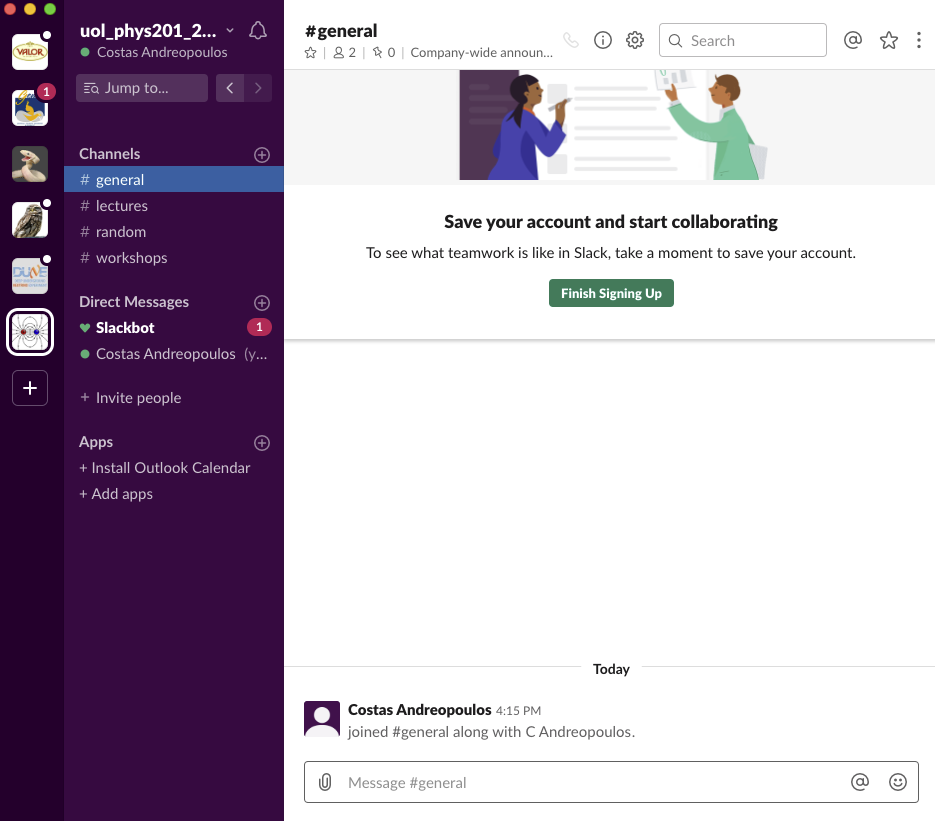
\includegraphics[width=0.50\textwidth]{./images/year_specific/phys201_slack_channel_201920.png}\\
\end{center}

Signup with your liverpool.ac.uk account at
{\color{blue} \url{https://join.slack.com/t/uolphys201201920/signup}}

\end{frame}

%
%
%

\begin{frame}{Lectures / Workshops / Assessment}

\begin{itemize}
\item {\bf One 2-hour lecture per week}
   \begin{itemize}
       \item Every Wedn. 11:00-13:00 (in CTH-LTC)
       \item Normally, 11 lectures in 2019 + revision lecture in Jan 2020
    \end{itemize}

\vspace{0.1cm}
\begin{block001}{Notice}
\begin{columns}
  \begin{column}{0.20\textwidth}
   \begin{center}
     
\includegraphics[width=0.25\textwidth]{./images/icons/warning.png}\\
   \end{center}
  \end{column}
  \begin{column}{0.80\textwidth}
  {\small
       {\bf \underline{Lectures start promptly at 11 am}}\\
       Please be on time and avoid disrupting the class.
   }
  \end{column}
\end{columns}
\end{block001}
\vspace{0.1cm}

\item {\bf One 2-hour workshop per week}
   \begin{itemize}
       \item Every Thurs. 11:00-13:00 (in CTL-4-FLEX)
       \item 10 workshops in total - {\color{red} Note: Starting in week \#2, not tomorrow!}
   \end{itemize}
\item Non-contact hours: 102 (average study time 8.5 hrs/week)
\item Credits: 15
\item Assessment:
   \begin{itemize}
      \item 2-hour examination (70\%)
      \item Workshops (30\%)
          \begin{itemize}
                \item 3 marked workshops (typically \#3, \#6, \#9) $\times$ 10\% each
          \end{itemize}
   \end{itemize}
\end{itemize}

\end{frame}


%
%
%

\begin{frame}{PHYS201 2019/20 calendar}

PHYS201 calendar (until further notice):\\
  \begin{center}
    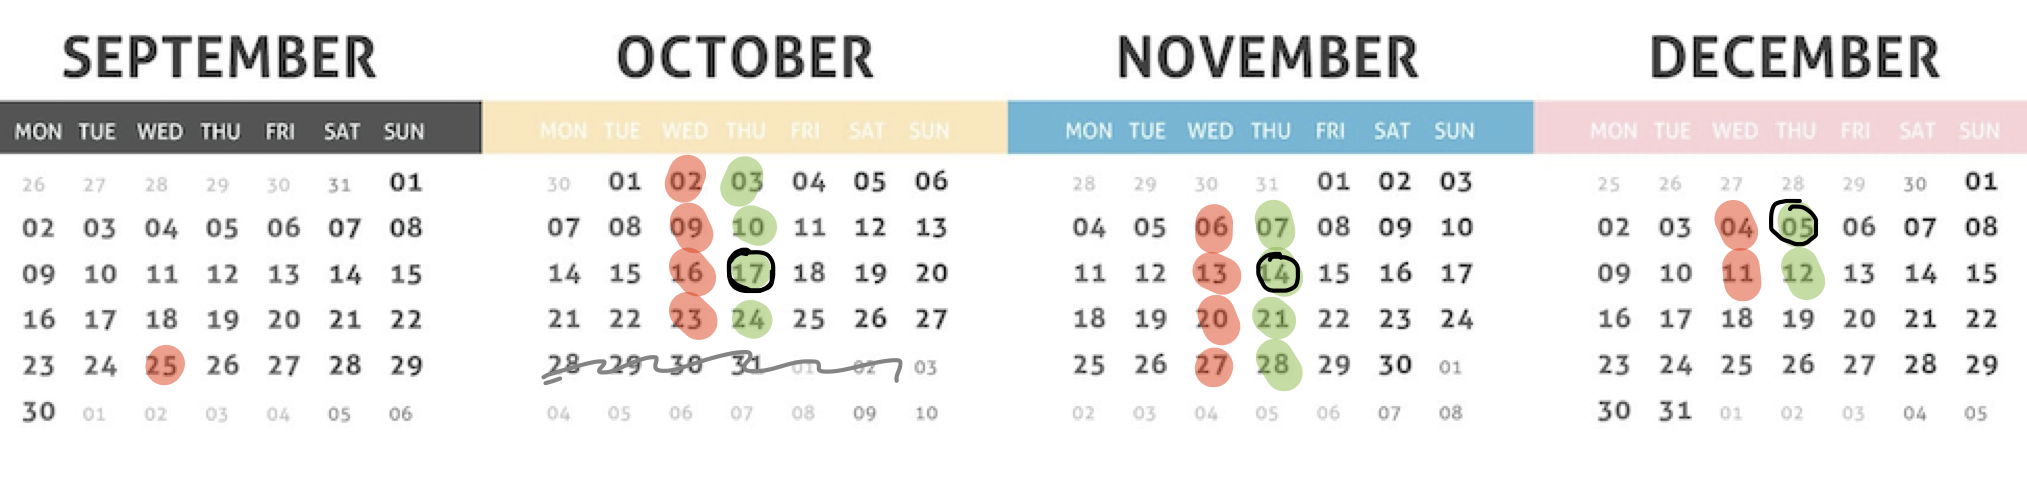
\includegraphics[width=0.95\textwidth]{./images/year_specific/phys201_calendar_201920_v1.png}\\
  \end{center}

\begin{itemize}
  \item red circles: 2-hr lecture slots
  \item green circles: 2-hr workshop slots
  \item highlighted green circles: assessed workshops (tentative, may change)
\end{itemize}

\end{frame}

%
%
%

\begin{frame}{Aims of the course}

\begin{itemize}
{\small
\item
To introduce the fundamental concepts and principles of electrostatics, magnetostatics,
electromagnetism and Maxwell's equations, and electromagnetic waves.
\item
To introduce differential vector analysis in the context of electromagnetism.
\item
To introduce circuit principles and analysis (EMF, Ohm's law, Kirchhoff's rules, RC and RLC circuits)
\item
To introduce the formulation of Maxwell's equations in the presence of dielectric and magnetic materials.
\item
To develop the ability of students to apply Maxwell's equations to simple problems involving dielectric and
magnetic materials.
\item
To develop the concepts of field theories in Physics using electromagnetism as an example.
\item
To introduce light as an electromagnetic wave.
}
\end{itemize}

\vspace{0.2cm}
\noindent\rule{2cm}{0.4pt}\\
{\it \scriptsize Source: PHYS 201 module page in ORBIT.}

\end{frame}

%
% Syllabus
%

\begin{frame}{Syllabus}

\begin{itemize}
{\small
\item
Electric charge, Coulomb’s law, Charge density
\item
Electric field, Principle of Superposition
\item
Electric flux, Gauss’ law (integral form)
\item
Mutual potential energy of point charges, electric potential
\item
Calculating the field from the potential (gradient)
\item
Circulation, charges on conductors
\item
Gauss’ law in differential form (divergence)
\item
Circulation law in differential form (curl)
\item
Poisson’s and Laplace’s laws and solutions
\item
Electric dipole
\item
Electrostatics and conductors, method of images
\item
Gauss’ and Stokes’ theorems
\item
EMF, potential difference, electric current, current density
\item
Resistance, Ohm’s law
\item
Circuits, Kirkhhoff’s rules
}
\end{itemize}

\end{frame}


\begin{frame}{Syllabus cont'd}

\begin{itemize}
{\small
\item
Capacitance, calculation of capacitance for simple cases, RC circuits
\item
Dielectrics, polarization, electric displacement field
\item
Capacitance in the presence of dielectrics, force on a dielectric
\item
Magnetism, magnetic field, Biot-Savart law
\item
Lorentz force, force between currents
\item
Charged particle motion in magnetic field, velocity filter
\item
Magnetic dipole field, Ampere’s law in integral and differential forms
\item
Maxwell’s equations in vacuum for steady conditions
\item
Vector potential
\item
Magnetic materials, magnetization, magnetic field strength
\item
Maxwell’s equations in the presence of materials for steady conditions
\item
Motion of conductors inside magnetic fields, Faraday’s and Lenz’s laws
\item
Time-varying fields, Maxwell’s equations for the most general case
\item
Derivation of electromagnetic waves from Maxwell’s equations, speed of light
\item
LCR circuits
}
\end{itemize}

\vspace{0.2cm}
\noindent\rule{2cm}{0.4pt}\\
{\it \scriptsize Source: PHYS 201 module page in ORBIT.}

\end{frame}

%
%
%

\begin{frame}{Our approach will be calculus based}

\begin{itemize}
{
      \item We will explore several {\bf interesting physics concepts}.
      \item Our approach will be calculus-based.
      \begin{itemize}
      {
         \item for an interesting alternative approach, see here:\\
                    {\color{blue} \tt http://videolectures.net/mit802s02\_electricity\_magnetism/}
      }
      \end{itemize}
      \item The electromagnetic phenomena are described by a set of {\bf very beautiful
                mathematical equations ({\em Maxwell} equations)}.
}
\end{itemize}


\begin{columns}
  \begin{column}{0.45\textwidth}
   \begin{center}
     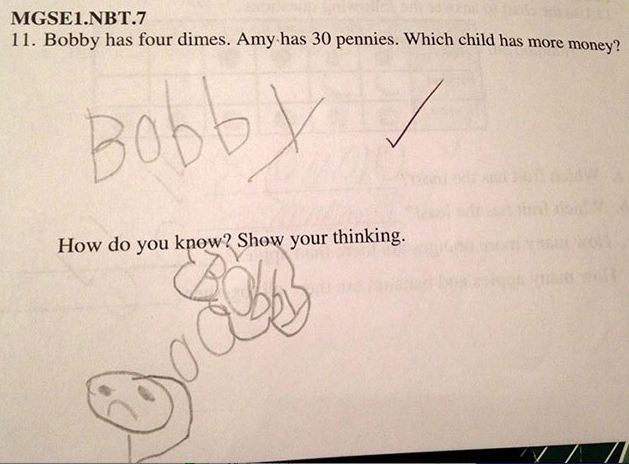
\includegraphics[width=0.80\textwidth]{./images/photos/bobby.png}\\
   \end{center}
  \end{column}
  \begin{column}{0.55\textwidth}
  {\small
         Mathematical dexterity necessary to
         \begin{itemize}
          { \small
                 \item sharpen your instinct
                 \item help you understand the connections between
                   different physics concepts
                  \item tackle practical problems
          }
         \end{itemize}
   }
  \end{column}
\end{columns}

\vspace{0.25cm}
{\bf Dust off your maths textbooks}! Its importance can not be overstated.\\

\end{frame}


%
%
%

\begin{frame}{Recommended textbooks}

Will follow mainly:
\begin{itemize}
    \item D.J. Griffiths, `Introduction to Electrodynamics', Prentice Hall, 1999\\
          {\it Paper copies available in the library.}
\end{itemize}

You may also find useful:
\begin{itemize}
{\footnotesize
    \item The Feynman Lectures in Physics\\
          Available online: {\it http://www.feynmanlectures.caltech.edu}
    \item L.S. Grant and W.R. Phillips, `Electromagnetism', Wiley, 2013\\
         {\it An ebook version available in the library.}
    \item W.J. Duffin, `Electricity and Magnetism', McGraw-Hill, 1990\\
          {\it Paper copies available in the library.}
    \item Daniel Fleisch, `A Student's Guide to Maxwell's Equations', Cambridge, 2008\\
         {\it Paper copies and an ebook version available in the library.}
    \item Daniel Fleisch, `A Student's Guide to Vectors and Tensors', Cambridge, 2011\\
         {\it Paper copies and an ebook version available in the library.}
    \item George Arfken, `Mathematical methods for physicists', Oxford, 2012\\
         {\it An ebook version available in the library.}
}
\end{itemize}

\end{frame}


%
%
%

\begin{frame}{Slides / Handouts}

There are 4 types of slides:
{\color{darkpowderblue} Blue}, {\color{dBG1} Red},
{\color{eBG1} Orange}, and {\color{pBG1} Green}.

\begin{columns}
  \begin{column}{0.50\textwidth}
   \begin{center}
     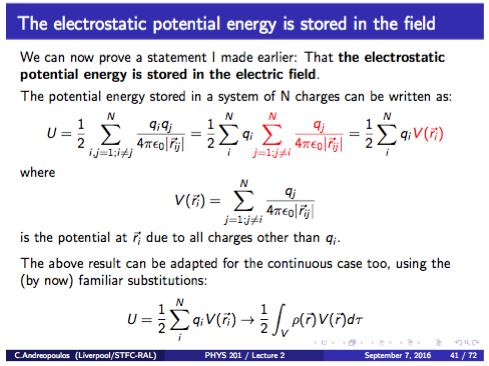
\includegraphics[width=0.7\textwidth]{./images/example_slides/main.png}\\
   \end{center}
  \end{column}
  \begin{column}{0.50\textwidth}
   \begin{center}
     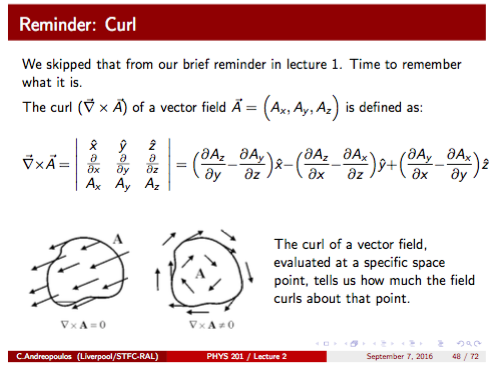
\includegraphics[width=0.7\textwidth]{./images/example_slides/reminder.png}\\
   \end{center}
  \end{column}
\end{columns}

\begin{columns}
  \begin{column}{0.50\textwidth}
   \begin{center}
     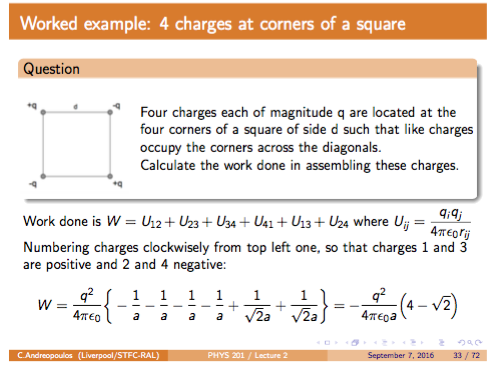
\includegraphics[width=0.7\textwidth]{./images/example_slides/worked_example.png}\\
   \end{center}
  \end{column}
  \begin{column}{0.50\textwidth}
   \begin{center}
     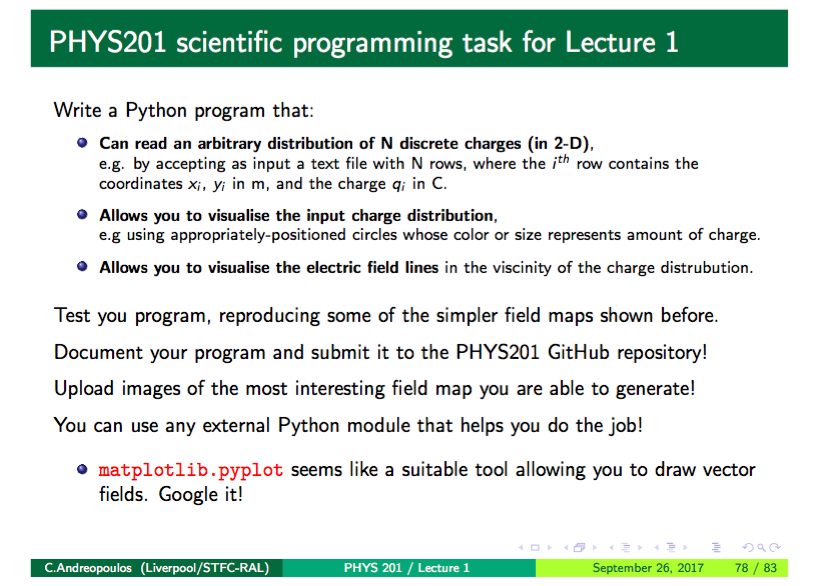
\includegraphics[width=0.7\textwidth]{./images/example_slides/python.png}\\
   \end{center}
  \end{column}
\end{columns}

\end{frame}


%
%
%

\begin{frame}{"Blue slides"}

\begin{columns}
  \begin{column}{0.30\textwidth}
   \begin{center}
        The main body of each PHYS201 lecture.\\
   \end{center}
  \end{column}
  \begin{column}{0.70\textwidth}
   \begin{center}
     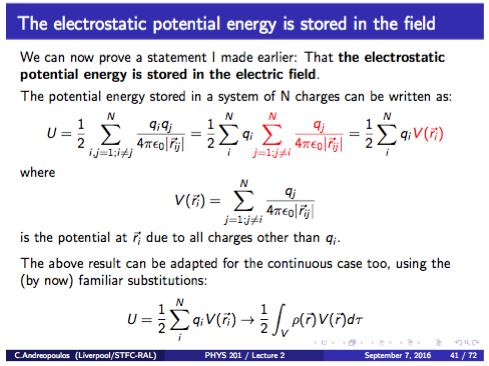
\includegraphics[width=0.99\textwidth]{./images/example_slides/main.png}\\
   \end{center}
  \end{column}
\end{columns}

\vspace{0.2cm}

\begin{center}
 {\bf Please check VITAL regularly for corrections and updates}.\\
\end{center}

\end{frame}

%
%
%

\begin{frame}{"Red slides"}

\begin{columns}
  \begin{column}{0.30\textwidth}
   \begin{center}
      Things you should already know / {\bf reminders}.\\
      \vspace{0.2cm}
      This material is here for easy reference!
      Typically, I will skip most of these slides during the lecture.\\
      \vspace{0.2cm}
      Please study the reminders in advance of each lecture.\\
   \end{center}
  \end{column}
  \begin{column}{0.70\textwidth}
   \begin{center}
     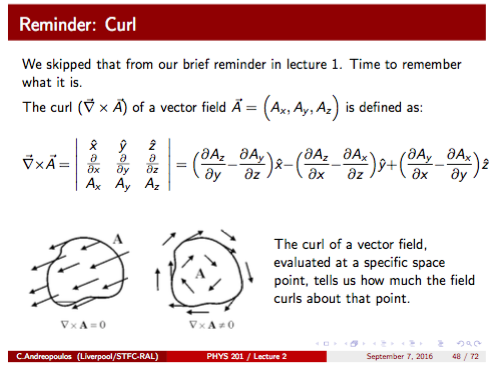
\includegraphics[width=0.99\textwidth]{./images/example_slides/reminder.png}\\
   \end{center}
  \end{column}
\end{columns}

\vspace{0.2cm}

\begin{center}
 {\bf Please check VITAL regularly for corrections and updates}.\\
\end{center}

\end{frame}


%
%
%


\begin{frame}{"Orange slides"}

\begin{columns}
  \begin{column}{0.30\textwidth}
   \begin{center}
      Questions and worked examples.\\
      \vspace{0.2cm}
      Will study as many as we have time for.
      More may be added in the digital version to address specific class needs.\\
   \end{center}
  \end{column}
  \begin{column}{0.70\textwidth}
   \begin{center}
     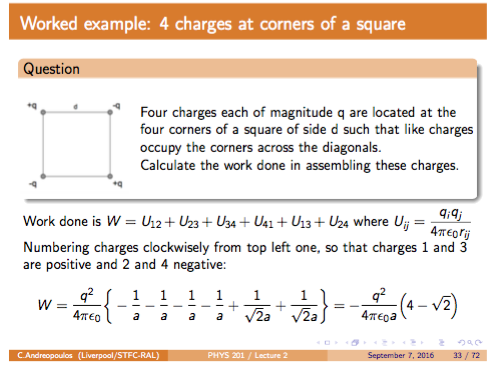
\includegraphics[width=0.99\textwidth]{./images/example_slides/worked_example.png}\\
   \end{center}
  \end{column}
\end{columns}

\vspace{0.2cm}

\begin{center}
 {\bf Please check VITAL regularly for corrections and updates}.\\
\end{center}

\end{frame}

%
%
%

\begin{frame}{"Green slides"}

\begin{columns}
  \begin{column}{0.52\textwidth}
     {\small
      Optional tasks (1/lecture) for which the analytical solution is too complex\\
      \vspace{0.2cm}
      Solve numerically, using C++/ROOT, Python or any other language (*)\\
      \vspace{0.2cm}
      Will be adding tasks, along with helpful hints, throughout the semester.\\
      \vspace{0.2cm}
      No marks awarded (optional tasks) but:
      \begin{itemize}
      {\scriptsize
        \item Improve your understanding of concepts!
        \item Gain experience in scientific computing!\\
      }
      \end{itemize}
     }
  \end{column}
  \begin{column}{0.48\textwidth}
   \begin{center}
     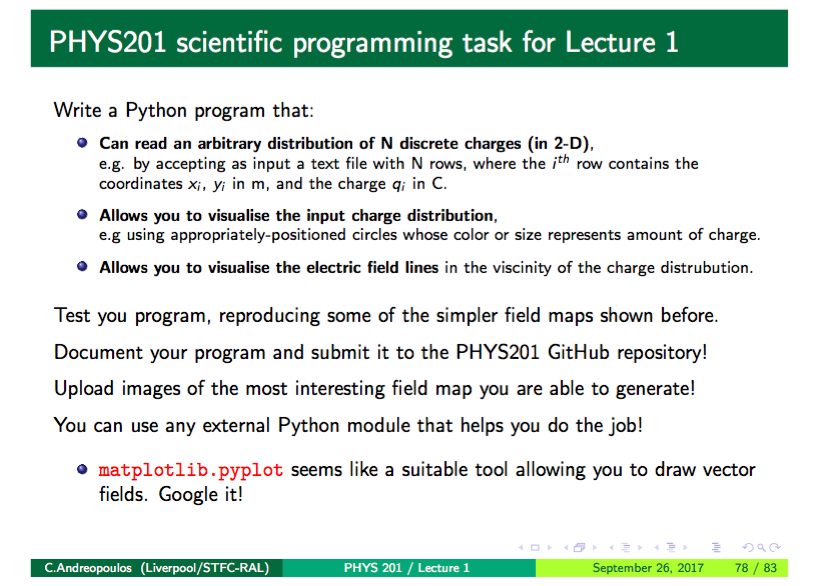
\includegraphics[width=0.99\textwidth]{./images/example_slides/python.png}\\
   \end{center}
  \end{column}
\end{columns}

\end{frame}

%
%
%

\begin{frame}{What is examinable?}

\begin{itemize}
  \item Everything that is in the PHYS201 slides \underline{is examinable}
  \begin{itemize}
      \item Unless I explicitly state otherwise
  \end{itemize}

  \vspace{0.3cm}

  \item Everything I discuss during the lectures (whether it is in the PHYS201 slides or not) \underline{is examinable}
  \begin{itemize}
      \item Unless I explicitly state otherwise
  \end{itemize}

  \vspace{0.3cm}

  \item Most of what I will discuss is in the slides, but not everything!

\end{itemize}


\begin{block001}{Notice}
\begin{columns}
  \begin{column}{0.15\textwidth}
   \begin{center}
     
\includegraphics[width=0.60\textwidth]{./images/icons/warning.png}\\
   \end{center}
  \end{column}
  \begin{column}{0.85\textwidth}
  {\small
     {\bf You should try and attend all lectures!}\\
     Stream Capture is available in this lecture theatre and used for all PHYS201 lectures.
   }
  \end{column}
\end{columns}
\end{block001}

\end{frame}

%
%
%

\begin{frame}{Getting feedback}

Don't expect written, personalised feedback delivered to your doorstep!\\
\vspace{0.3cm}
Take control of your own learning and seek feedback - there are
{\bf numerous opportunities} to do so.
\vspace{0.2cm}
\begin{itemize}
  {\scriptsize
     \item At lecture, speak up and interrupt me at any moment with questions,
           or come and find me at the break.\\
     \item At the workshop, engage the TAs and me, and get detailed verbal
           feedback on your solutions.\\
     \item Bring in my attention workshop problems you would like to
           see discussed in detail during the lecture
           (in addition to the usual worked examples).\\
     \item Compare your solutions with model solutions (available on VITAL)
           and detailed marking scheme.\\
     \item Seek feedback from your peers, during the workshops and your study time.
     \item Visit me during my office hours or book an appointment.
     \item Send me an e-mail with your questions, or use the PHYS201 slack channel.\\
  }
  \end{itemize}

\end{frame}

%
%
%

\begin{frame}{Workshops}

\begin{itemize}
{\small
\item 10 workshops, 3 of which will be assessed
\item Tentatively, workshops 3,6,9 will be assessed (will confirm at the lecture prior to the assessed workshop)
\item I will collect your scripts only on the assessed workshops
\item Standard penalty applies for late submissions
\item Will aim to return the marked scripts within 2 weeks
\item It is easy to cheat, and a few students choose to attend
      only the assessed ones. Make no mistake: You will regret this during the final exam.
\vspace{0.2cm}
\item Workshop tasks will be made available {\bf several days} in advance.
\item Usually, too many tasks for 2 hours
\begin{itemize}
  \item Do not want to hear any complaint!!
  \item You have ample time to work on the problems {\bf before} the workshop
  \item Work on the problems in advance, and use the workshop as an opportunity to get feedback
        (rather than trying frantically to solve the problems for the first time)
\end{itemize}
\item Model solutions and a marking scheme will be made available shortly after the workshop.
}
\end{itemize}

\end{frame}

%
%
%

\begin{frame}{Fundamental forces}

\underline{Main goal of physics}:
Study of the {\bf fundamental constituents of matter and of the forces between them}.\\
\vspace{0.2cm}

\begin{columns}
  \begin{column}{0.60\textwidth}
   \begin{center}
     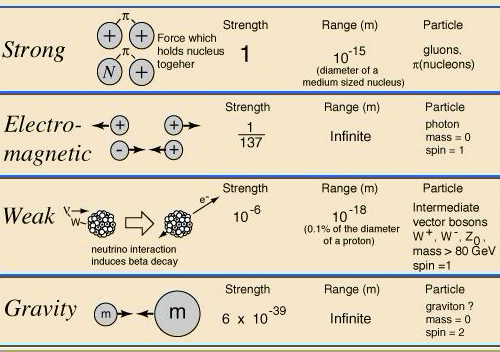
\includegraphics[width=0.98\textwidth]{./images/schematics/fundamental_forces.png}\\
   \end{center}
  \end{column}
  \begin{column}{0.40\textwidth}
    \begin{itemize}
    {\small
      \item Strong nuclear: keeps the atomic nucleus together
      \item {\color{magenta}Electromagnetism: the subject of this course.}
      \item Weak nuclear: responsible for nuclear $\beta$ decays
      \item Gravity: Pins you down on the Earth and rotates you around the Sun
    }
    \end{itemize}
  \end{column}
\end{columns}

\end{frame}

%
%
%

\begin{frame}{Electromagnetism}

\begin{center}
{\Large
Electromagnetism \\ {\bf shapes our environment and our perception of it.}\\
\vspace{0.3cm}
It {\bf underpins life} and \\ {\bf governs the processes that underpin chemistry}.\\
}
\end{center}
\end{frame}


\begin{frame}{Electromagnetism}

You see me because {\bf light (an electromagnetic wave)} was scattered off me
and interacted with photo-sensitive tissue in the retina of your eyes.\\
The response of that tissue is also electromagnetic:
{\bf Electrical impulses} traveled to your brain via the optic nerve.\\

\begin{center}
   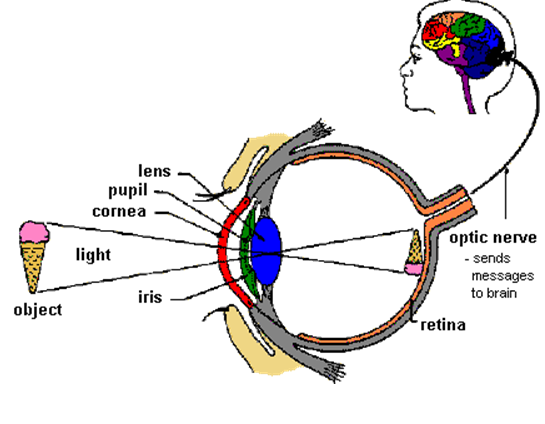
\includegraphics[width=0.50\textwidth]{./images/misc/vision_1.png}\\
\end{center}

\end{frame}

%
%
%

\begin{frame}{Electromagnetism}

\begin{columns}
  \begin{column}{0.50\textwidth}
  {
     If you hit your hand on your desk what you actually feel is an {\bf electromagnetic force},
     the {\bf repulsion between the electron clouds} in your hand and in your desk.\\
  }
  \end{column}
  \begin{column}{0.50\textwidth}
   \begin{center}
     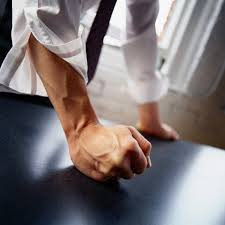
\includegraphics[width=0.80\textwidth]{./images/misc/hit_hand_on_desk.jpg}\\
   \end{center}
  \end{column}
\end{columns}

\end{frame}

%
%
%

\begin{frame}{Electromagnetism}

The contraction of the muscles in your heart caused by
{\bf electrical impulses} from the sinoatrial node.

\begin{center}
   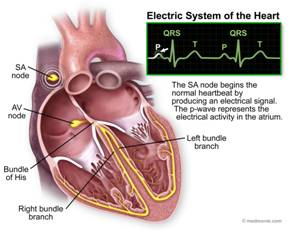
\includegraphics[width=0.65\textwidth]{./images/misc/electrical_system_heart.jpg}\\
\end{center}

\end{frame}

%
%
%

\begin{frame}{Electromagnetism}

\begin{center}
 {\bf Electric and magnetic forces known from ancient times.}\\
\end{center}

\begin{columns}
  \begin{column}{0.40\textwidth}
   \begin{center}
      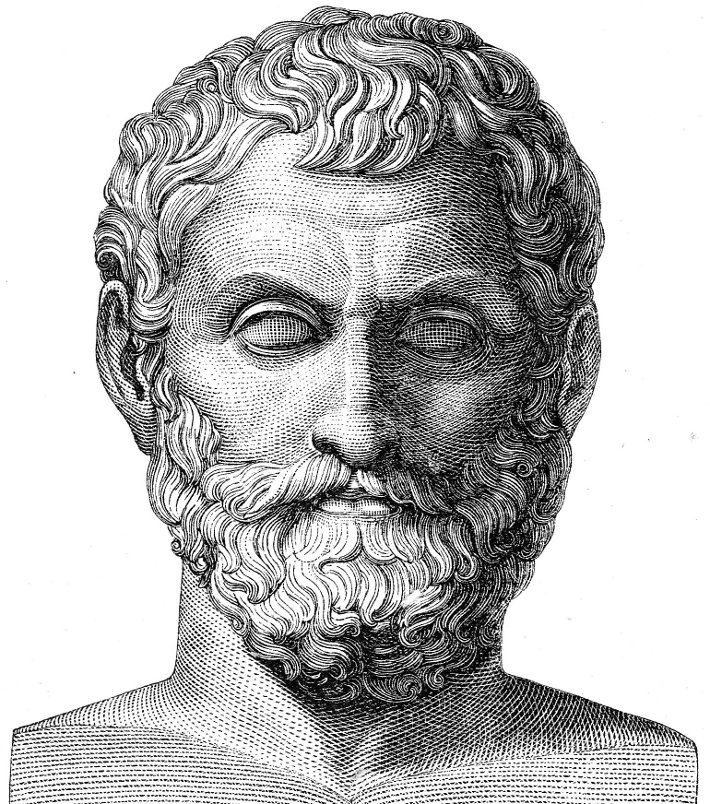
\includegraphics[width=0.80\textwidth]{./images/people/thales.jpg}\\
   \end{center}
  \end{column}
  \begin{column}{0.60\textwidth}
     Thales ($\sim$625-545 BC), a Greek Philosopher from Miletus (Asia Minor)
     has recorded observations of the properties of
     \begin{itemize}
       \item {\bf amber} and
       \item {\bf lodestones}.
     \end{itemize}
  \end{column}
\end{columns}

\end{frame}

%
%
%

\begin{frame}{Electromagnetism}

\begin{columns}
  \begin{column}{0.35\textwidth}
   \begin{center}
      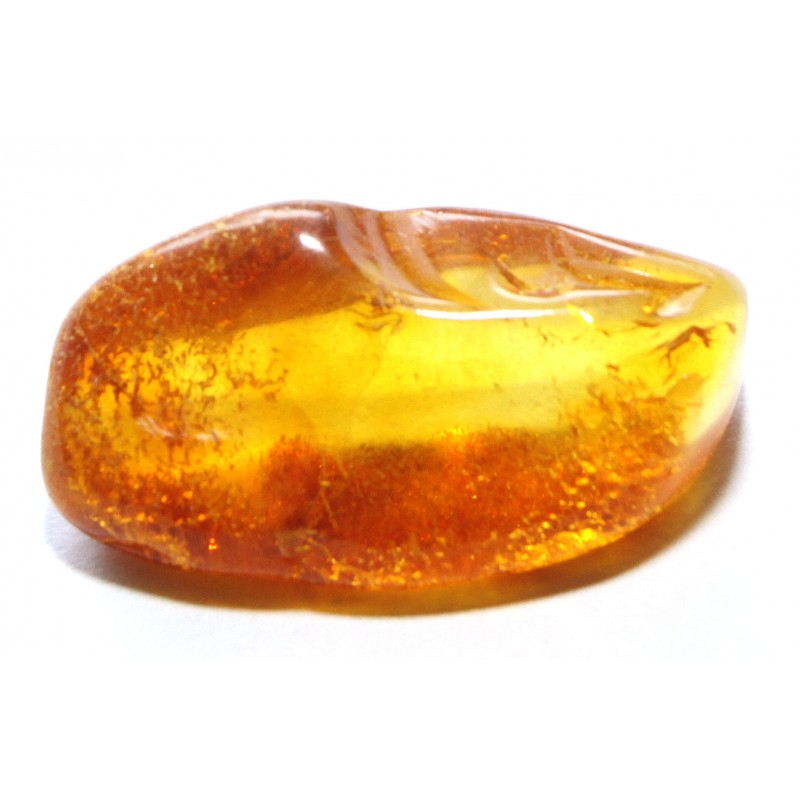
\includegraphics[width=0.95\textwidth]{./images/photos/amber_stone_1.jpg}\\
   \end{center}
  \end{column}
  \begin{column}{0.65\textwidth}
   \begin{itemize}
   {\small
    \item {\bf Amber}: a yellow-orange-brown fossilised tree resin
     \begin{itemize}
     {\scriptsize
        \item Amber is known as {\em `electron'} in Greek, the name given to first
              charged particle discovered and the origin of the term {\em electricity}.
     }
     \end{itemize}
     \item When rubbed with fur, amber could attract small bodies like small pieces of straw.
   }
   \end{itemize}
  \end{column}
\end{columns}

\vspace{0.1cm}

\begin{columns}
  \begin{column}{0.35\textwidth}
   \begin{center}
      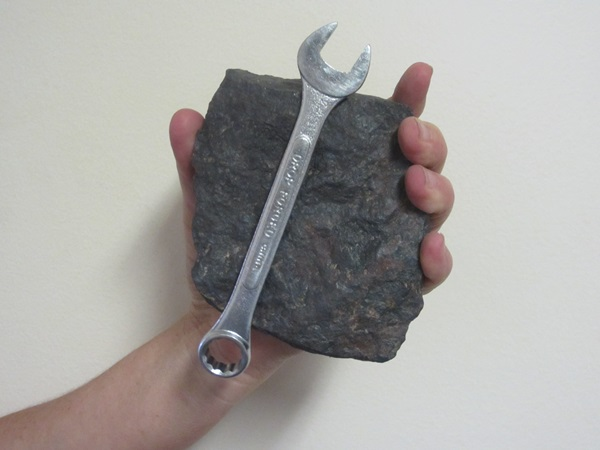
\includegraphics[width=0.90\textwidth]{./images/photos/lodestone_1.jpg}\\
   \end{center}
  \end{column}
  \begin{column}{0.65\textwidth}
   \begin{itemize}
    {\small
     \item {\bf Lodestone}: naturally magnetised piece of the mineral magnetite
     \begin{itemize}
     {\scriptsize
       \item Lodestones were first found in the Greek colony of {\em Magnesia},
             in what is now Asia minor, hence the term {\em magnetism}.
     }
     \end{itemize}
     \item Lodestone are attracted to iron and other lodestones.
    }
    \end{itemize}
  \end{column}
\end{columns}

\end{frame}


%
%
%

\begin{frame}{Electromagnetism}

{\bf Electric and magnetic forces had an impact on early thinking}.\\
\begin{itemize}
   \item Electricity and magnetism perplexed Thales: How can an (inanimate) object attract other objects?
   \item This led him to believe that amber and lodestone may be alive?
     \begin{itemize}
        \item And then, perhaps, everything is living.\\
     \end{itemize}
\end{itemize}

\vspace{0.3cm}

There were some early applications
\begin{itemize}
   \item Magnetic compass (Chinese, 12th century AD; others)
\end{itemize}

\vspace{0.3cm}

But no further advance in understanding till the early modern period.
\begin{itemize}
    \item William Gilbert (1540-1603)
\end{itemize}

\end{frame}

%
%
%

\begin{frame}{Electromagnetism}

\begin{itemize}

   \item The subject as we know it was {\bf developed in less than a century}
   \begin{itemize}
      \item $\sim$1785: Coulomb publishes his law
      \item $\sim$1864: Maxwell publishes his famous theory
        \begin{itemize}
            \item unity of electric and magnetic phenomena and understanding of light
        \end{itemize}
   \end{itemize}

   \item Several applications followed the development of the theory
   \begin{itemize}
     \item 1880: first wired-up house
     \item 1891: electric fan
     \item 1901: vacuum cleaner
     \item 1909: washing machine and iron
     \item 1918: refrigerator and dishwasher
     \item ...
   \end{itemize}
\end{itemize}

\begin{center}
  {\bf Try to imagine your life without electricity}!
\end{center}

\end{frame}

%
%
%

\begin{frame}{Electromagnetism}

It is a wonderful example of a {\bf {\em covariant} theory}
\begin{itemize}
  \item The {\bf Special theory of relativity} had its origins in Classical Electrodynamics
\end{itemize}

\vspace{0.2cm}

Classical Electrodynamics coupled with Quantum Mechanics gives rise to {\bf Quantum Electrodynamics (QED)}
\begin{itemize}
  \item Experimentally tested to 1 in $10^{11}$ parts
  \begin{itemize}
     \item 1 in $10^{11}$: Like predicting the distance from New York to Los Angeles to about half the thickness of usual printer paper...
  \end{itemize}
  \item {\bf One of the most successful theories} ever built, and the most precisely tested one in the history of science.
  \item A prototype for other Quantum Field Theories
\end{itemize}

\end{frame}
